\documentclass{article}

\usepackage{fancyhdr}
\usepackage{extramarks}
\usepackage{amsmath}
\usepackage{amsthm}
\usepackage{amsfonts}
\usepackage{tikz}
\usepackage[plain]{algorithm}
\usepackage{algpseudocode}
\usepackage{enumerate}

\usetikzlibrary{automata,positioning}

%
% Basic Document Settings
%

\topmargin=-0.45in
\evensidemargin=0in
\oddsidemargin=0in
\textwidth=6.5in
\textheight=9.0in
\headsep=0.25in

\linespread{1.1}

\pagestyle{fancy}
\lhead{\hmwkAuthorName}
\chead{\hmwkClass\ (\hmwkClassInstructor\ \hmwkClassTime): \hmwkTitle}
\rhead{\firstxmark}
\lfoot{\lastxmark}
\cfoot{\thepage}

\renewcommand\headrulewidth{0.4pt}
\renewcommand\footrulewidth{0.4pt}

\setlength\parindent{0pt}

%
% Create Problem Sections
%

\newcommand{\enterProblemHeader}[1]{
    \nobreak\extramarks{}{Problem \arabic{#1} continued on next page\ldots}\nobreak{}
    \nobreak\extramarks{Problem \arabic{#1} (continued)}{Problem \arabic{#1} continued on next page\ldots}\nobreak{}
}

\newcommand{\exitProblemHeader}[1]{
    \nobreak\extramarks{Problem \arabic{#1} (continued)}{Problem \arabic{#1} continued on next page\ldots}\nobreak{}
    \stepcounter{#1}
    \nobreak\extramarks{Problem \arabic{#1}}{}\nobreak{}
}

\setcounter{secnumdepth}{0}
\newcounter{partCounter}
\newcounter{homeworkProblemCounter}
\setcounter{homeworkProblemCounter}{1}
\nobreak\extramarks{Problem \arabic{homeworkProblemCounter}}{}\nobreak{}

%
% Homework Problem Environment
%
% This environment takes an optional argument. When given, it will adjust the
% problem counter. This is useful for when the problems given for your
% assignment aren't sequential. See the last 3 problems of this template for an
% example.
%
\newenvironment{homeworkProblem}[1][-1]{
    \ifnum#1>0
        \setcounter{homeworkProblemCounter}{#1}
    \fi
    \section{Problem \arabic{homeworkProblemCounter}}
    \setcounter{partCounter}{1}
    \enterProblemHeader{homeworkProblemCounter}
}{
    \exitProblemHeader{homeworkProblemCounter}
}

%
% Homework Details
%   - Title
%   - Due date
%   - Class
%   - Section/Time
%   - Instructor
%   - Author
%

\newcommand{\hmwkTitle}{Tutorial 1}
\newcommand{\hmwkDueDate}{January 19, 2021}
\newcommand{\hmwkClass}{CZ2003}
\newcommand{\hmwkClassTime}{SS3}
\newcommand{\hmwkClassInstructor}{Assoc Prof Alexei Sourin}
\newcommand{\hmwkAuthorName}{\textbf{Pang Yu Shao}}
\newcommand{\hmwkAuthorID}{\textbf{U1721680D}}

%
% Title Page
%

\title{
    \vspace{2in}
    \textmd{\textbf{\hmwkClass:\ \hmwkTitle}}\\
    \normalsize\vspace{0.1in}\small{Due\ on\ \hmwkDueDate\ at 10:30am}\\
    \vspace{0.1in}\large{\textit{\hmwkClassInstructor\ - \hmwkClassTime}}
    \vspace{3in}\\
    \hmwkAuthorName\\
    \hmwkAuthorID
}

\date{18/01/2021}

\renewcommand{\part}[1]{\textbf{\large Part \Alph{partCounter}}\stepcounter{partCounter}\\}

%
% Various Helper Commands
%

% Useful for algorithms
\newcommand{\alg}[1]{\textsc{\bfseries \footnotesize #1}}

% For derivatives
\newcommand{\deriv}[1]{\frac{\mathrm{d}}{\mathrm{d}x} (#1)}

% For partial derivatives
\newcommand{\pderiv}[2]{\frac{\partial}{\partial #1} (#2)}

% Integral dx
\newcommand{\dx}{\mathrm{d}x}

% Alias for the Solution section header
\newcommand{\solution}{\textbf{\large Solution}}

% Probability commands: Expectation, Variance, Covariance, Bias
\newcommand{\E}{\mathrm{E}}
\newcommand{\Var}{\mathrm{Var}}
\newcommand{\Cov}{\mathrm{Cov}}
\newcommand{\Bias}{\mathrm{Bias}}

\begin{document}

\maketitle

\pagebreak

\begin{homeworkProblem}
    A straight line is defined by equation \(y = 3x + 4\) in Cartesian 
    coordinate system \(XY\)
   

    \begin{enumerate}[i]
        \item Define this straight line in polar coordinates \(r, a\) as
            an explicit function \(r = f(a)\)
        \item Specify the domain for the polar coordinate \(a\) in both
              radians and degrees for this straight line.
    \end{enumerate}

    \textbf{Solution}\\
    \textbf{Part i}\\
    Recall the conversion between \(x,y\) to \(r\)
    \begin{itemize}
        \item \(x = rcos(a)\)
        \item \(y = rsin(a)\)
    \end{itemize}
    \[
        \begin{split}
            y  &= 3x + 4
            \\
            rsin(a) &= 3rcos(a) + 4 
            \\
            rsin(a) - 3rcos(a) &= 4
            \\
            r(sin(a) - 3cos(a)) &= 4
            \\
            \mathbf{r} &= \mathbf{4 / (sin(a) - 3cos(a))}
            \\
        \end{split}
    \]



    \textbf{Part ii}\\
    Domain of \(a\) is not continuous as r will be undefined when denominator equates to 0:\\
    
    \[
        \begin{split}
            sin(a) - 3cos(a)  &= 0
            \\
            sin(a) &= 3cos(a) 
            \\
            tan(a) &= 3
            \\
            a &= tan^{-1}(3)
            \\
            &= 1.249\ or\ \pi+1.249
            \\
            &= 1.249\ or\ 4.391\ (radians)
            \\
            &= 71.57^{\circ}\ or\ 251.56^{\circ}\ (degrees)
            \\
        \end{split}
    \]

    \begin{itemize}
        \item \textit{Radians}: \(a \in (1.249, 4.391)\)
        \item \textit{Degrees}: \(a \in (71.57^{\circ}, 251.56^{\circ})\)
    \end{itemize}



\end{homeworkProblem}

\pagebreak
\begin{homeworkProblem}
    \begin{enumerate}[i]
        \item Define in polar coordinates \(r = f(a)\) the origin-centred 
              circle with radius \(R\). Specify the domain for the polar coordinate \(a\)
        \item Define in polar coordinates \(r = f(a)\) a circle with radius \(R\) 
              and the centre at the Cartesian coordinates \((R,0)\). 
              Specify the domain for the polar coordinate \(a\)
    \end{enumerate}
    \textbf{Solution}\\
    \textbf{Part i}\\
    For a circle centred at the origin with radius \(R\), the circle can be defined 
    in polar co-ordinates by:\\\\
    \begin{center}
    \(r = R,  a \in [0, 2\pi)\)
    \end{center}
    \textbf{Part ii}\\
    For a circle centred at \((R,0)\) with radius \(R\), the circle can be defined 
    in cartesian co-ordinates using the following equation:
    \begin{center}
        \((x-h)^{2} + (y-k)^{2} = r^{2}\)
    \end{center}
    where,
    \begin{itemize}
        \item \(h\) is the x-coordinate of centre of circle
        \item \(k\) is the y-coordinate of centre of circle
        \item \(r\) is the radius of the circle 
    \end{itemize}

    In this case we have:
    \begin{center}
        \((x-R)^{2} + (y)^{2} = R^{2}\)
    \end{center}

    Substituting 
    \begin{itemize}
        \item \(x = rcos(a)\)
        \item \(y = rsin(a)\)
    \end{itemize}
    We get:
    \begin{center}
        \((rcos(a)-R)^{2} + (rsin(a))^{2} = R^{2}\)\\
        \(r^{2}cos^{2}(a)-2R*rcos(a) + R^{2} + r^{2}sin^{2}(a) = R^{2}\)\\
        \(r^{2}cos^{2}(a)-2R*rcos(a) + r^{2}sin^{2}(a) = 0\)\\
        \(r^{2}cos^{2}(a) + r^{2}sin^{2}(a) = 2R * rcos(a)\)\\
        \(r(sin^{2}(a) + cos^{2}(a)) = 2Rcos(a)\)\\
    \end{center}
    Since \(sin^{2}(a) + cos^{2}(a) = 1\),
    \begin{center}
        \(r = 2Rcos(a)\)\\
    \end{center}

    Thus, for a circle centred at \((R,0)\) with radius \(R\), the circle can be defined 
    in polar co-ordinates by:\\\\
    \begin{center}
    \(r = 2Rcos(a),  a \in [-0.5\pi, 0.5\pi]\)
    \end{center}
    
\end{homeworkProblem}

\pagebreak

\begin{homeworkProblem}
    With reference to Figure \ref{fig/Q3}, write formulas deriving 
    Cartesian coordinates \(x, y, z\), from the cylindrical \(r, \alpha, h\) and spherical 
    coordinates \(r, \alpha, \beta\). Notice that the axes layout is different in the two cases.
    \begin{figure}[H]
        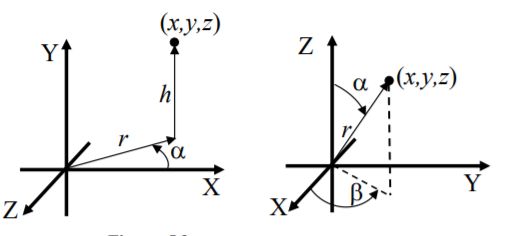
\includegraphics[width=6cm]{fig/q3.PNG}
        \centering
        \caption{Reference figures for converting between Cartesian to 
        cylindrical and spherical coordinates}
        \label{fig/Q3}
    \end{figure}

    \textbf{Solution}\\
    \textbf{Converting from Cylindrical to Cartesian Coordinates}\\
    At first glance, we can easily to derive \(y\) from \(y\):
    \begin{center}
        \(\mathbf{y = h}\)
    \end{center}
    Next, \(x\) and \(z\) can be derived from \(r\) and \(\alpha\) like converting
    from 2-dimensional cartesian coordinates to polar coordinates.\\

    However, it is worth noting that in this case, z-axis is in place of the 
    typical y-axis and the z-axis is also flipped. Therefore, we arrive at the 
    following derivations:
    \begin{center}
        \(\mathbf{x = rcos(\alpha)}\)\\
        \(\mathbf{y = h}\)\\
        \(\mathbf{z = -rsin(\alpha)}\)\\

    \end{center}

    \textbf{Converting from Spherical to Cartesian Coordinates}\\
    For converting from spherical coordinates to cartesian coordinates, We look at the projection
    of R on the \(XY\) plane. Let this projection be \(\mathbf{p}\)
    \begin{figure}[H]
        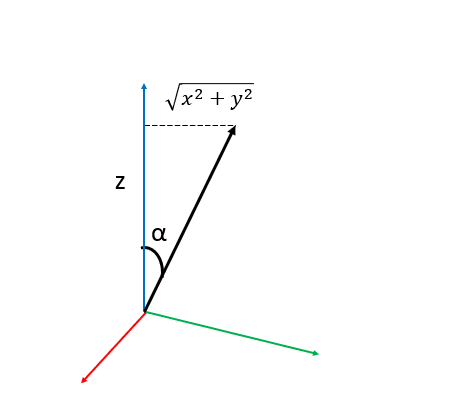
\includegraphics[width=6cm]{fig/q3_1.PNG}
        \centering
    \end{figure}
    We can obtain the following equations:
    \begin{center}
        \(\mathbf{z = rcos(\alpha)}\)\\
        \(p = rsin(\alpha)\)\\
    \end{center}

    With the projection of p, we can then get the following
    \begin{center}
        \(x = pcos(\beta)\)\\
        \(y = psin(\beta)\)\\
    \end{center}

    Which allows us to arrive at the derivations:
    \begin{center}
        \(\mathbf{x = rsin(\alpha)cos(\beta)}\)\\
        \(\mathbf{y = rsin(\alpha)sin(\beta)}\)\\
        \(\mathbf{z = rcos(\alpha)}\)\\
    \end{center}


\end{homeworkProblem}

\pagebreak
\begin{homeworkProblem}
    \begin{enumerate}[i]
        \item With reference to Figure \ref{fig/Q4}, calculate coordinates (numbers) of the unit
        (magnitude is equal to 1) normal vector N.
        \item What are the coordinates of the unit normal vector to the opposite side
        of the triangle?
    \end{enumerate}
    \begin{figure}[H]
        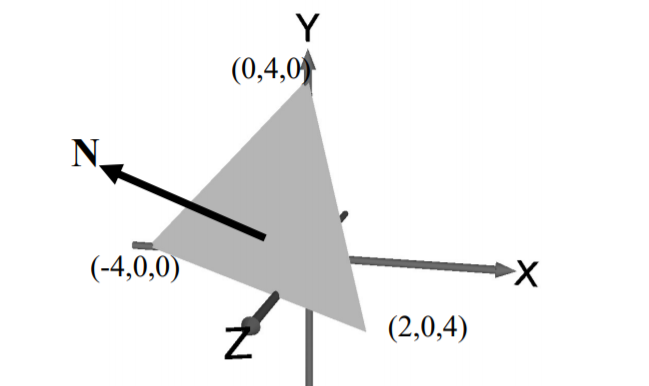
\includegraphics[width=6cm]{fig/q4.PNG}
        \centering
        \caption{Reference figure for finding Unit Normal Vector from surface}
        \label{fig/Q4}
    \end{figure}
    
\end{homeworkProblem}

\textbf{Solution}\\
\textbf{Part i}\\
To find the normal vector N, we define two other vectors, \(v_1\) and \(v_2\):
\begin{figure}[H]
    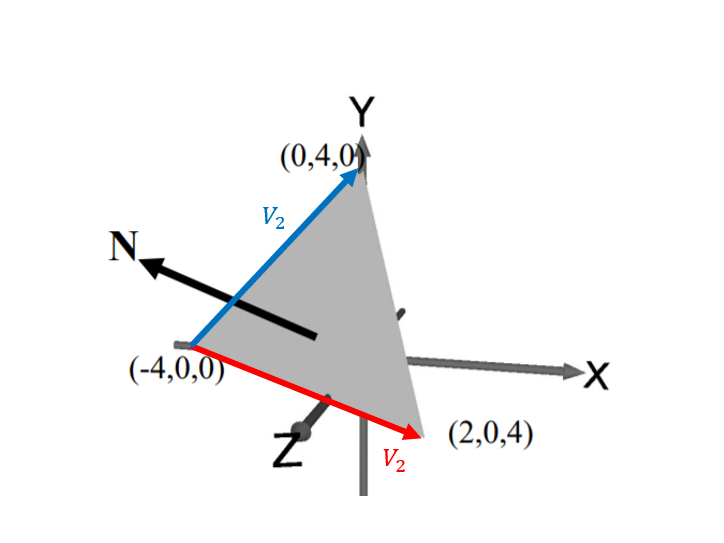
\includegraphics[width=8cm]{fig/q4_1.PNG}
    \centering
\end{figure}

The vector Normal to the surface can then be found by obtaining the cross product of the
two vectors, \(N = v_1 \times v_2\)

\[
        \begin{split}
            v1 &= [(2 - (-4))\ (0 - 0)\ (4 - 0)]
            \\
            &= [6\ 0\ 4]
            \\
            v2 &= [(0 - (-4))\ (4 - 0)\ (0 - 0)]
            \\
            &= [4\ 4\ 0]
            \\\\
            N &= v1 \times v2
            \\
            &= [(0*0)-(4*4)\ (4*4)-(6*0)\ (6*4)-(0*4)]
            \\
            &= [-16\ 16\ 24]
            \\\\
            ||N|| &= \sqrt{(-16)^{2} + 16^{2} + 24^{2}}
            \\
            &= 8\sqrt{17}
            \\\\
            Unit\ Normal\ Vector, N_n &= \left[\frac{-16}{8\sqrt{17}}\ \frac{16}{8\sqrt{17}}\ \frac{24}{8\sqrt{17}}\right]
            \\
            &= \left[\frac{-2}{\sqrt{17}}\ \frac{2}{\sqrt{17}}\ \frac{3}{\sqrt{17}}\right]
        \end{split}
    \]

    \textbf{Part ii}\\
    To get coordinates of Unit Normal Vector to the opposite side of the triangle, we can apply a scale of \(-1\)
    to the vector obtained in \textbf{Part i}.

    \[
        \begin{split}
        (-1)(N_n) &= \left[-1*\frac{-2}{\sqrt{17}}\ -1*\frac{2}{\sqrt{17}}\ -1*\frac{3}{\sqrt{17}}\right]
        \\
        &= \left[\frac{2}{\sqrt{17}}\ \frac{-2}{\sqrt{17}}\ \frac{-3}{\sqrt{17}}\right]
        \end{split}
    \]
    



\end{document}